%
% File acl2020.tex
%
%% Based on the style files for ACL 2020, which were
%% Based on the style files for ACL 2018, NAACL 2018/19, which were
%% Based on the style files for ACL-2015, with some improvements
%%  taken from the NAACL-2016 style
%% Based on the style files for ACL-2014, which were, in turn,
%% based on ACL-2013, ACL-2012, ACL-2011, ACL-2010, ACL-IJCNLP-2009,
%% EACL-2009, IJCNLP-2008...
%% Based on the style files for EACL 2006 by 
%%e.agirre@ehu.es or Sergi.Balari@uab.es
%% and that of ACL 08 by Joakim Nivre and Noah Smith

\documentclass[11pt,a4paper]{article}
\usepackage[hyperref]{acl2020}
\usepackage{times}
\usepackage{graphicx}
\usepackage{latexsym}
\usepackage{fancyvrb}
\usepackage{subcaption}

\renewcommand{\UrlFont}{\ttfamily\small}

% This is not strictly necessary, and may be commented out,
% but it will improve the layout of the manuscript,
% and will typically save some space.
\usepackage{microtype}
\usepackage[natbib=false]{biblatex} 
\addbibresource{acl2020.bib}

\aclfinalcopy % Uncomment this line for the final submission
%\def\aclpaperid{***} %  Enter the acl Paper ID here

%\setlength\titlebox{5cm}
% You can expand the titlebox if you need extra space
% to show all the authors. Please do not make the titlebox
% smaller than 5cm (the original size); we will check this
% in the camera-ready version and ask you to change it back.

\newcommand\BibTeX{B\textsc{ib}\TeX}

\title{Image Classification}

\author{Alex Rasla \\
  UC Santa Barbara \\
  \texttt{alexrasla@ucsb.edu}}

\date{February 2, 2022}

\begin{document}
\maketitle

\section{Data}

For this project, I used the CIFAR-10 \cite{Krizhevsky09learningmultiple} dataset which consists of 60,000 32x32 images, 
 split into 50,000 for training and 10,000 for testing. In order to gain more diverse dataset/images
  and train a model more robust model, I implemented a data augmentation technique on this dataset that
  included random horizontal flipping and random cropping.

\section{Libraries}

In this project, I used Pytorch to create my CNN and Torchvision to download and perform transformations on the CIFAR-10 dataset.
 Within PyTorch, I used Conv2d layers to perform convolutions, ReLU layers to ensure all values are $>=$ 0, BatchNormalization as a 
 regularization technique, and MaxPool2d layers to reduce the dimensions of the image and extract the most important features. I used the 
 Torchvision library to download the CIFAR-10 dataset and transform the images rather than manually loading and 
 processing the data everytime into my project. Lastly, I used NumPy for basic array operations, matplotlib for
  plotting metrics, and sklearn to generate a confusion matrix.


\section{Models}
To perform and experiment with different image classification techniques, I first created a baseline model to ensure I could 
achieve reasonable image classification. This model consisted of 3 layers of convolution followed by a “classification” layer. 
Each of the convolutional layers had kernel sizes of 3, maxpooling sizes of 2, and consisted of the following sequential components: 
Conv2d, ReLU, Conv2d, ReLU, and MaxPool2d; the final classification layer consisted of the Flatten, Linear, ReLU, Linear, ReLU, 
Linear sequential components, with a final output vector size of 10. This model was trained with a learning rate of 0.001, a batch size of 100, 
over 30 epochs, using the cross entropy loss function.

Once I trained and produced reasonable results for a simple model, I also decided to train a larger model with the first and last 
layers consisting of the convolutional layers described above, and 3 layers in between consisting of a sequential Conv2d, ReLU, Conv2d,
 ReLU, Conv2d, ReLU, and MaxPool2d. This model was trained with the same hyperparameters as the baseline one in order to be able to compare 
 them as accurately as possible.

 
\section{Implementation Details}

In order to train an image classification model using my program, first connect to the \href{https://colab.research.google.com/}{Google Colab} GPU 
and clone \href{https://github.com/alexrasla/ImageClassification.git}{my repository}.
Next, to edit the model type and its hyperparameters, change the values in the config.py. Finally, execute 
\begin{Verbatim}[fontsize=\small]
  !python3 ./ImageClassification/train.py
\end{Verbatim}
 to train the image classification model specificied in the MODEL variable in the Config class.
Once this model is trained, evaluation can be performed by executing: 
 \begin{Verbatim}[fontsize=\small]
  !python3 ./ImageClassification/eval.py 
                 --model [path to model]
 \end{Verbatim}
The evaluation is performed on the CIFAR-10 testset, and the program generates and saves a 
confusion matrix, which is used to plot and analyze the results using 
\begin{Verbatim}[fontsize=\small]
  !python3 ./ImageClassification/plot.py 
         --dir [path to model directory]
\end{Verbatim}

\section{Results}

Throughout this project, I trained two different models, experimented with a variety of different hyperparameters,
 and tested out different regularization and data augmentation techniques to achieve the most accurate model. In order 
 to compare the models, I used the most common evaluation techniques for image classification models: a confusion matrix. 
 This matrix increments the index of model's output label (row) and the ground truth label (column) in the confusion matrix for each test image. Using this
 method, perfect accuracy is represented by a diagonal matrix. However, more notable metrics using this matrix are the 
 overall accuracy, the commission of error, and the omission of error. The overall accuracy is percentage of correct 
 predictions, the commission of error is the percentage of images that are assigned to a certain class that don't belong 
 to it (overestimation), and the omission of error is the percentage of images that belong to one class but are classified by the model 
 as other classes (underestimation). A table of the overall accuracy, training time per epoch, and validation time per epoch 
 for each model I trained and experimented with is shown in Table \ref{tab:table1}. The training and validation loss for the best model (Model A)
 are shown in Figure \ref{fig:plots}, its normalized confusion matrix is shown in Figure \ref{fig:confusion}, and its error of commission
  and omission are shown in Figure \ref{fig:commission_omision}.

Contrary to my initial hypothesis, the smaller model with fewer layers and convolutions had a better overall accuracy as compared to the larger model 
 when trained with the same hyperparamters and data. This was a novel realization for myself because I always assumed larger models perform better. However, after reading 
 various research papers, I found that this is in fact expected the expected behavior in CNNs used for image classification. 

The best performing model I was able to train achieved an overall accuracy of 0.8912, a final training loss of 0.127, a final validation loss of 0.441 as shown in Figure \ref{fig:plots}, and a total training time of 23 minutes and 33 seconds.
  As we can see from the confusion matrix in Figure \ref{fig:confusion}, most of the model's classification accuracies lied above 0.89. From the commision and omision bar graph
   \ref{fig:commission_omision}, we also notice that the two classes below this threshold, cat and dog, seemed to be most difficult task for the model, and were often hard to differentiate between themselves.
   In fact, $9\%$ of the commision and ommision errors for each of these classes were caused by the other. Nevertheless, the model performed very well on the other classes, with half the classes
   above $90\%$ accuracy.

%This model converged continuously for the first 5-10 epochs, and the gradually converged for the remaining 20-25. I noticed that training for more epochs than 30 lead to
  % model overfitting and a diverging validation loss.  

 \begin{table}
    \centering
    \begin{tabular}{ |c|c|c|c| } 
     \hline
      & Overall Accuracy & Train & Validation \\
     \hline
     Model A & 0.8912 & 42.42 & 5.04 \\ 
     \hline
     Model B & 0.8605 & 34.98 & 2.09 \\ 
     \hline
     Model C & 0.8378 & 91.26 & 5.29 \\ 
     \hline
     Model D & 0.7895 & 41.60 & 3.05 \\ 
     \hline
     Model E & 0.7773 & 98.42 & 5.03 \\ 
     \hline
     Model F & 0.6612 & 83.38 & 5.17 \\ 
     \hline
     Model G & 0.6556 & 45.13 & 3.35 \\ 
     \hline
    
    \end{tabular}
    \caption{Model A: Small, Data Augmentation, Batch Normalization; Model B: Small, 30 epochs, Data Augmentation; Model C: Large, 30 epochs, Data Augmentation;
    Model D: Small, 20 epochs, 3x3 Kernels; Model E: Large, 20 epochs, 3x3 Kernels; Model F: Small, 20 epochs, 7x7 Kernels;
    Model G: Small, 40 epochs, 3x3 Kernels. This figure shows the overall accuracy from the confusion matrix 
    for each trained model, along with its average training and validation time in seconds per epoch.}
    \label{tab:table1}
\end{table}

\begin{figure}
  \centering
  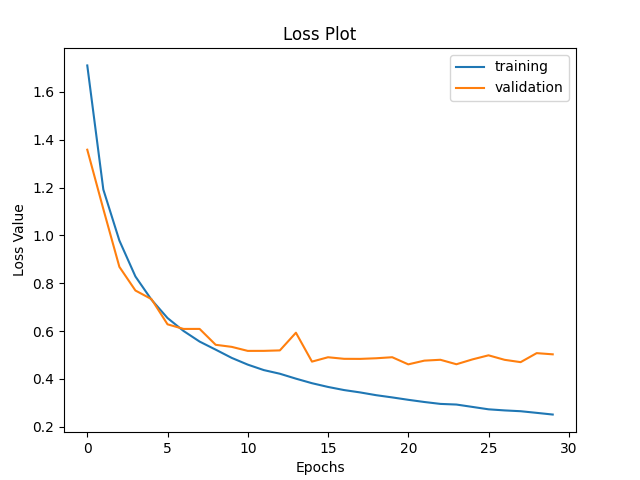
\includegraphics[width=0.40\textwidth]{figures/plots.png}
  \caption{The training and validation loss plots for Model A: Small, Data Augmentation, Batch Normalization}
  \label{fig:plots}
\end{figure}

\begin{figure}
  \centering
  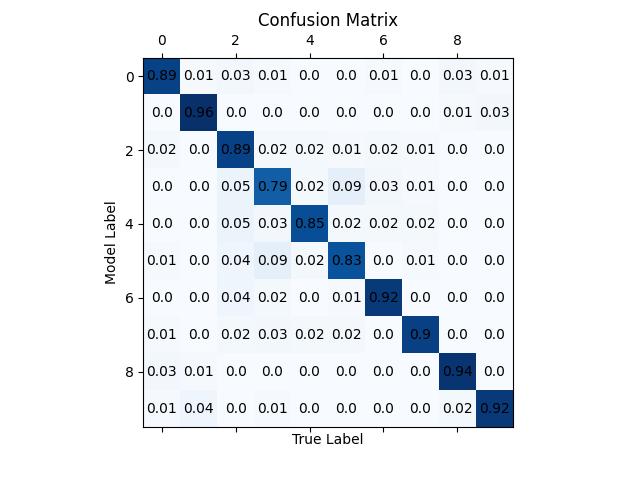
\includegraphics[width=0.40\textwidth]{figures/confusion.png}
  \caption{The confusion matrix for Model A}
  \label{fig:confusion}
\end{figure}

\begin{figure}
  \centering
  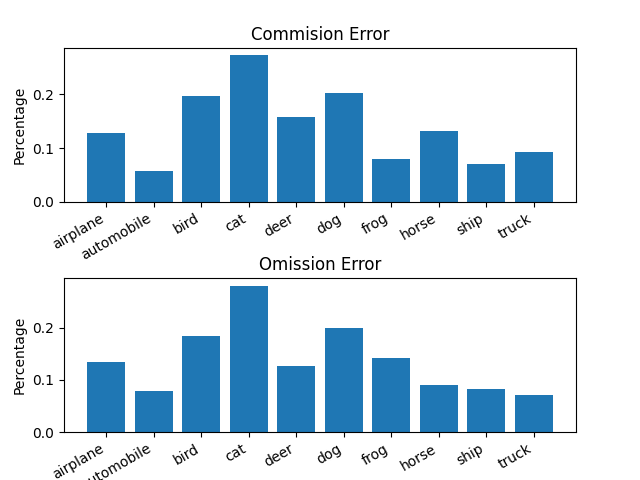
\includegraphics[width=0.40\textwidth]{figures/commission_omision.png}
  \caption{The commission and omision of error for Model A}
  \label{fig:commission_omision}
\end{figure}



\section{Discussion}

For my experimentation in this project, I implemented two different models (one large, one small),
 and analyzed the effect of different kernel sizes, number of epochs, learning rate, data augmentation, and regularization techniques. 
 In order to perform this experimentation, I first trained the smaller model that is described in the model section. 
 This model gave me insight into how accurate a CNN can be without any hyperparameter tuning or modifications. 
 I trained this model for 20 epochs with a learning rate of 0.001 and a kernel size of 3x3. This produced an overall 
 accuracy of 0.7895 for the CIFAR-10 testset. 

Once this smaller model generated reasonable results, I decided to test whether or not a larger model (Model E) with 
 more layers and convolutions would increase the performance and accuracy. I trained the model with identical hyperparameters
  in order to be able to most effectively compare the smaller and larger model. Contrary to my hypothesis, this did not perform
   better than its simpler counterpart --- it achieved an overall accuracy of 0.7773. Furthermore, this model took twice as long
    to train and was 1GB in size (compared to 67MB for the small model) because of the number of trainable parameters. 

Because I noticed a slight decrease in performance with the larger model (and a huge increase in size), I decided to build upon and experiment
 with the smaller model. I first experimented with a kernel size of 7x7 (and a padding size of 3 so every pixel can be processed).
  This model performed noticeably worse than the smaller model with 3x3 kernels, decreasing the overall accuracy to 0.6612.
   This is likely because the images in the CIFAR-10 dataset are only 32x32. Using a 7x7 kernel for convolutions for images this 
   small makes it hard for the model to extract important features and characteristics; the features that differentiate the images
    from each other and allow them to be classified correctly are smaller and more detailed. In other words, a smaller kernel size 
    can better specify and recognize a pixel's relation to a classification rather than a bigger kernel size which has a harder 
    time determining these details and relationships.

Next, I experimented with the number of epochs and learning rate for the smaller model to see if tuning these hyperparameters 
 would improve performance. In order to test this, I trained the smaller model for 40 epochs with a learning rate of 0.0005.
  This would run the data over the entire dataset twice as much, but update the model's weights by half as much as the original 
  model. Unfortunately, changing these parameters also drastically decreased the performance again to an overall accuracy of 0.6556, 
  but maintained a similar train and validation time per epoch. This is likely because the model overfitted the training data, 
  and thus performed poorly on the testing and validation data. This was proven by the diverging validation loss, as well as the 
  poor overall accuracy.

My last attempt at improving the model itself was to use regularization techniques since the dataset is relatively small and
 they are proven to improve many types of models for many types of applications. I decided to focus on experimenting with dropout 
 layers and batch normalization. Throughout my experimentation with a dropout of 0.15, I noticed that even one dropout layer in 
 the neural network prevented the model from converging \italics at all. This was very surprising to me since I thought regularization 
 techniques can only improve model performance, given they are not overused. I suspect it failed to improve performance because dropping 
 convolution weights with a kernel size of 3 are already small enough that dropping additional neurons is ineffective and prevents it
  from learning. On the other hand, batch normalization after convolutional layers proved to increase the model's overall performance
  to by 0.03. This is likely because standardizing the output of the convolutional layers prevents overfitting the model to the training set.

Finally, I decided to experiment with data augmentation. In order to perform data augmentation, the CIFAR-10 images I used needed
 to be modified in some way to diversify the dataset. To modify the images, I used torchvision's transform module to randomly flip 
 the images horizontally with $p=0.5$ and randomly crop the image. These transformations ensured the model was able to find more robust 
 features that represented a certain image classification rather than simply learning the dataset and overfitting the data. As a 
 result of this data augmentation, the overall accuracy of the smaller model improved by nearly 0.08, and the accuracy of the large 
 model improved nearly 0.05. This is a significant improvement from the initial models, which truly shows the impact that data 
 augmentation has on improving image classification.

Building upon the smaller model with the combination of batch normalization and data augmentation, I was able to improve the
 model's overall accuracy by 0.1, or $10\%$, to 0.8912.


\printbibliography

\end{document}
